%% DATA 226 Term Project Report
%% Template: IEEE Computer Society journal (IEEEtran, compsoc option),
%% as in the Overleaf "IEEE demo template for computer science journals".
\documentclass[10pt,journal,compsoc]{IEEEtran}

\usepackage[nocompress]{cite}
\usepackage{amsmath}
\usepackage{graphicx}
\usepackage{booktabs}
\usepackage{array}
\usepackage{tabularx}
\usepackage{xcolor}
\usepackage{tikz}
\usetikzlibrary{arrows.meta,positioning,fit,shapes.geometric}
\usepackage{pgfplots}
\pgfplotsset{compat=1.17}
\usepackage{url}
\usepackage[hidelinks]{hyperref}

% Placeholder marker for parts the team still has to complete
\newcommand{\todo}[1]{\textcolor{red}{\textbf{[TEAM: #1]}}}

\begin{document}

\title{Streaming Attribution of Lightning-Caused Wildfire Ignitions: A Kafka--Spark--MongoDB Pipeline for the August 2020 California Lightning Siege}

\author{Group 7: Rachel Huang, Pablo Nguyen, Chinmayi Bolisetty, and Anastasiia Gogoleva%
\IEEEcompsocitemizethanks{\IEEEcompsocthanksitem DATA 226, Department of Applied Data Intelligence, San Jos\'e State University.\protect\\
Code and data: \url{https://github.com/chinmayibolisetty-cmd/wildfire-lightning-pipeline.}}}

\markboth{DATA 226 Project Report, Fall 2026}{Streaming Attribution of Lightning-Caused Wildfire Ignitions}

\IEEEtitleabstractindextext{%
\begin{abstract}
Lightning ignited hundreds of fires in California within a few days in August 2020, and many of them burned for weeks. Attributing a newly detected fire to the lightning that likely caused it is a streaming problem: two high-velocity satellite feeds must be joined in space and time while the data arrive. We built and evaluated an end-to-end pipeline that replays NOAA GOES-17 Geostationary Lightning Mapper (GLM) flashes and NASA FIRMS VIIRS fire detections through Apache Kafka, joins them with Spark Structured Streaming, and stores matches in MongoDB with geospatial indexes. A detection counts as a new fire if no other detection lies within 5\,km in the previous 7 days, and it is attributed to lightning if a flash occurred within $D$\,km and $T$\,h before it. Using 60,803 flashes, 44,022 fire detections, and 242 lightning fires recorded in the USDA FPA FOD database for Aug 15--22, 2020, we show that real lightning matches new fires 1.5 times more often than a spatially shifted chance baseline, that the lightning filter raises precision against ground truth from 23\% to 38\%, and that 8 of the 15 largest recorded fires, covering 56\% of their burned area, were attributed to lightning. Against CAL FIRE fire perimeters as a second ground truth, over an extended window of Aug 15--25, the filter raises precision from 46\% to 76\%, and 16 of 18 large lightning fires were detected. Both rules run inside the stream: a stateful Spark query detects new fires and a second query joins them with lightning, reproducing the batch prototype exactly (139 of 139 new fires, 65 of 65 matches) at up to 30,959 events/s with a median end-to-end latency of 7.1--7.5\,s. A 2dsphere index cut MongoDB query time from 36.6\,ms to 0.57\,ms, against 346\,ms for the same lookup in Snowflake. We also applied five techniques from the course: a Bloom filter detects new fires in one pass with 36 times less memory than an exact set, Flajolet--Martin estimates distinct struck cells within 8.8\% on average, locality-sensitive hashing finds all matched fires while examining 0.18\% of flashes, differential privacy quantifies the cost of releasing noisy fire counts, and a data-poisoning test shows that requiring three flashes keeps precision near 34--39\% when fake flashes are injected.
\end{abstract}

\begin{IEEEkeywords}
Stream processing, Apache Kafka, Spark Structured Streaming, spatio-temporal join, Bloom filter, locality-sensitive hashing, differential privacy, MongoDB, wildfire, lightning, GOES GLM, VIIRS.
\end{IEEEkeywords}}

\maketitle
\IEEEdisplaynontitleabstractindextext
\IEEEpeerreviewmaketitle

%% ===================================================================
\section{Introduction}
\IEEEPARstart{O}{n} August 16, 2020, a band of dry thunderstorms crossed Northern and Central California and started hundreds of fires within days. Several grew into the August, LNU Lightning, SCU Lightning, North, and SQF complexes, which together burned more than two million acres. During such an event, fire managers must decide quickly which new fire detections are lightning ignitions, because lightning fires appear in clusters, often in remote terrain, and can smoulder for days before they are seen (``holdover'' fires~\cite{moris2023holdover,kalashnikov2023liw}).

Two satellite systems observe both halves of the problem continuously. The GOES-17 Geostationary Lightning Mapper (GLM) reports lightning flashes over the Western Hemisphere every 20 seconds~\cite{goodman2013glm}, and the VIIRS instrument detects active fires at 375\,m resolution about twice a day~\cite{schroeder2014viirs}, distributed through NASA FIRMS. Joining these feeds is a classic Big Data velocity problem: events arrive continuously, a match requires both a spatial and a temporal condition, and the time window must be long (tens of hours) because of holdover.

This project builds and evaluates a streaming pipeline for this task. Our contributions are:
\begin{itemize}
\item An end-to-end, containerized pipeline (Kafka, Spark Structured Streaming, MongoDB) that replays real GLM and FIRMS data, detects new fires with per-cell Spark state, and performs a spatio-temporal stream--stream join using a spatial grid to avoid an all-pairs comparison.
\item A statistical check of the attribution against a chance baseline, including a flawed first baseline that we identified and replaced.
\item An evaluation against two ground truths, the USDA FPA FOD records~\cite{short2022fpafod} and CAL FIRE fire perimeters~\cite{calfire2020perimeters}, including a precision/recall sweep over the distance and time parameters, an extended window, and a fire-by-fire check of the largest fires and complexes.
\item Throughput, latency, and index benchmarks showing that the streaming job reproduces the batch result exactly, and a comparison of MongoDB with the Snowflake data warehouse.
\item Measured applications of course techniques to the same data: a Bloom filter and Flajolet--Martin sketch, locality-sensitive hashing, differential privacy, and a data-poisoning robustness test.
\end{itemize}

%% ===================================================================
\section{Literature Survey}

\subsection{Lightning Observation from Space}
GLM is a staring optical imager on the GOES-R series that detects total lightning (in-cloud and cloud-to-ground) day and night with near-uniform coverage of the Americas~\cite{goodman2013glm}. Its pixel size is about 8\,km at nadir, growing toward the edge of the field of view, which bounds how precisely a flash can be placed relative to a fire. GLM Level~2 files group optical events into groups and flashes and are published every 20 seconds. Rudlosky \textit{et al.}~\cite{rudlosky2025lightningfire} recently compared flashes known to have ignited western U.S. wildfires in 2020--2022 with non-igniting flashes using ground-based network and GLM data, and found that igniting flashes produced notably brighter GLM signals.

\subsection{Satellite Active-Fire Detection}
The VIIRS 375\,m active-fire product~\cite{schroeder2014viirs} improves on the 1\,km MODIS product in detecting small and low-intensity fires and is available in near real time through NASA FIRMS. Each detection carries a time, location, confidence class, and fire radiative power. Because the polar-orbiting Suomi NPP satellite overpasses a location about twice a day, there is an inherent delay of up to roughly 12 hours between a fire becoming visible and its first detection.

\subsection{Attributing Fires to Lightning and Holdover Time}
Most lightning--fire attribution studies search for lightning within a spatial buffer around a fire's ignition point and a backward time window from its discovery~\cite{moris2023holdover}. Larjavaara \textit{et al.}~\cite{larjavaara2005finland} introduced a proximity index that combines the distance and time between flash and fire. Moris \textit{et al.}~\cite{moris2023holdover} compiled a global database of holdover times and reported medians between 1.4 and 53.6 hours, with most distributions having a majority of fires detected within 24 hours. Kalashnikov \textit{et al.}~\cite{kalashnikov2023liw} showed that western U.S. holdover fires detected 2--5 days after ignition occurred under wetter conditions than promptly detected fires. These studies motivate our time window $T$ and show that attribution is inherently uncertain. They are batch analyses of historical records; none processes the satellite feeds as streams.

\subsection{Ground-Truth Wildfire Records}
The Fire Program Analysis Fire-Occurrence Database (FPA FOD)~\cite{short2022fpafod} harmonizes 2.3 million U.S. wildfire records from federal, state, and local agencies for 1992--2020, including discovery date, final size, point of origin, and a standardized cause. It is the standard ground truth for U.S. fire-cause studies and the source of our evaluation labels. CAL FIRE's Fire and Resource Assessment Program compiles California fire perimeters with alarm date, size and cause~\cite{calfire2020perimeters}; unlike a single point of origin, a perimeter records the whole burned area.

\subsection{Stream Processing Systems}
Apache Kafka~\cite{kreps2011kafka} is a distributed, partitioned commit log that decouples producers from consumers and allows streams to be replayed. Discretized Streams~\cite{zaharia2013dstreams} brought fault-tolerant micro-batch processing to Spark, and Structured Streaming~\cite{armbrust2018structured} expresses streaming computations as incremental queries over unbounded tables, with event-time watermarks that bound the state kept for stream--stream joins. These watermarks are what make a 48-hour join window feasible.

\subsection{Spatial Data Management}
Distributed spatial frameworks such as GeoSpark (now Apache Sedona)~\cite{yu2015geospark} partition data spatially so that joins compare only nearby objects. We apply the same idea with a fixed grid inside a standard Spark job. On the storage side, MongoDB's 2dsphere index supports spherical geometry queries such as ``all points within a radius''~\cite{mongodb2dsphere}.

\subsection{Streaming Algorithms}
The course text~\cite{leskovec2020mmds} covers algorithms for bounded-memory stream processing. A Bloom filter~\cite{bloom1970} answers set-membership queries in constant space with no false negatives; Kirsch and Mitzenmacher~\cite{kirsch2006lesshashing} showed that two hash functions suffice to simulate $k$ of them. The Flajolet--Martin sketch~\cite{flajolet1985} estimates the number of distinct elements in a stream from the longest run of trailing zeros in hashed values, and LogLog counting~\cite{durand2003loglog} refined how several such estimates are averaged.

\subsection{Similarity Search, Privacy, and Robustness}
Locality Sensitive Hashing~\cite{indyk1998lsh} finds near neighbours without comparing all pairs; the p-stable scheme of Datar \textit{et al.}~\cite{datar2004pstable} applies it to Euclidean distance with random projections. K-anonymity~\cite{sweeney2002kanon} and differential privacy~\cite{dwork2006dp} protect individuals in released data; the Laplace mechanism~\cite{dwork2006calibrating} adds noise scaled to a query's sensitivity. Data poisoning, in which an attacker injects crafted training or input data, was demonstrated by Biggio \textit{et al.}~\cite{biggio2012poisoning}; we adapt the idea to injected sensor events.

\subsection{Gap Addressed}
To our knowledge, no openly available system joins GLM and VIIRS as live streams, checks the result against a chance baseline, and validates it against FPA FOD. Our pipeline does all three on a real, extreme event.

%% ===================================================================
\section{Data}

Table~\ref{tab:data} summarizes the four datasets. We restricted all data to a California bounding box (32.5--42.0$^\circ$N, 124.5--114.0$^\circ$W).

\begin{table}[!t]
\caption{Datasets Used}
\label{tab:data}
\centering
\footnotesize
\setlength{\tabcolsep}{3pt}
\begin{tabular}{@{}p{4.3cm}lr@{}}
\toprule
Dataset & Window (2020) & Records \\
\midrule
GOES-17 GLM L2 flashes & Aug 15--20 & 60,803 \\
\quad extension & Aug 21--25 & 36,948 \\
\quad source files (20\,s each) & & $\approx$47,500 \\
FIRMS VIIRS S-NPP (standard processing) & Aug 8--25 & 44,022 \\
\quad nominal/high confidence & & 41,647 \\
FPA FOD natural-cause fires, CA & 2019--2020 & 1,096 \\
\quad discovered Aug 15--22 & & 242 \\
\quad \ldots of which $\geq$10 acres & & 60 \\
\quad discovered Aug 15--25 & & 268 \\
CAL FIRE fire perimeters, CA & 2020 & 503 \\
\quad lightning, started Aug 13--27 & & 51 \\
\bottomrule
\end{tabular}
\end{table}

\textbf{Lightning.} GLM Level~2 files were read anonymously from NOAA's public cloud bucket; we kept flash time, latitude, longitude, energy, and area. Fig.~\ref{fig:daily} shows that lightning peaked on Aug 16--17 (15,894 and 16,489 flashes) with a second peak on Aug 19. For the broader evaluation (Section~\ref{sec:broad}) we later added Aug 21--25 (36,948 flashes), which shows a second lightning episode building over Aug 23--25.

\textbf{Fires.} FIRMS detections were requested through the FIRMS area API in five-day chunks. The week before Aug 15 serves only as history for the new-fire rule. Daily detections rose from about 120 per day before the siege to 10,663 on Aug 19 (Fig.~\ref{fig:daily}), which shows the burst in velocity that a streaming system must absorb. We dropped low-confidence detections.

\textbf{Ground truth.} From FPA FOD we kept California fires from 2019--2020 whose general cause is ``Natural''. Of these, 242 were discovered between Aug 15 and Aug 22, 2020, and 182 of them (75\%) burned less than 10 acres.

\textbf{Perimeters.} From CAL FIRE's compilation of fire perimeters we downloaded the 503 perimeters for 2020 in California, each with a cause and alarm date. Of these, 51 are lightning fires (cause code 1) that started between Aug 13 and Aug 27, and 18 of them burned at least 1,000 acres. A first attempt with the NIFC history layer returned only 12 small perimeters and none of the siege complexes.

\begin{figure}[!t]
\centering
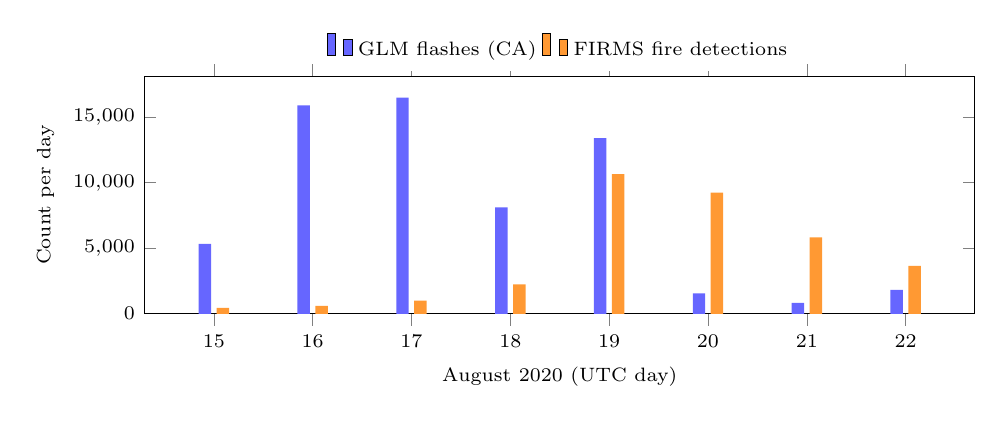
\begin{tikzpicture}
\begin{axis}[
  width=\columnwidth, height=4.6cm,
  ybar, bar width=4.5pt,
  symbolic x coords={15,16,17,18,19,20,21,22},
  xtick=data, xlabel={August 2020 (UTC day)},
  ylabel={Count per day}, ymin=0,
  legend style={at={(0.5,1.02)},anchor=south,legend columns=2,font=\scriptsize,draw=none},
  tick label style={font=\scriptsize}, label style={font=\scriptsize},
  scaled y ticks=false,
  yticklabel style={/pgf/number format/fixed},
]
\addplot[fill=blue!60,draw=none] coordinates {(15,5341) (16,15894) (17,16489) (18,8127) (19,13400) (20,1552) (21,822) (22,1825)};
\addplot[fill=orange!80,draw=none] coordinates {(15,457) (16,602) (17,1005) (18,2251) (19,10663) (20,9245) (21,5831) (22,3663)};
\legend{GLM flashes (CA), FIRMS fire detections}
\end{axis}
\end{tikzpicture}
\caption{Daily lightning flashes and fire detections (all confidence levels). Aug 21--22 lightning comes from the extension used in Section~\ref{sec:broad}. Fire detections peak two to three days after the lightning peak.}
\label{fig:daily}
\end{figure}

%% ===================================================================
\section{System Design and Methods}\label{sec:methods}

\subsection{Overall Flow}
Fig.~\ref{fig:flow} shows the logical flow. Download scripts turn the raw archives into three clean CSV files. A replay producer publishes flashes and fire detections to two Kafka topics in event-time order at a configurable speed-up. Two Spark Structured Streaming queries follow: the first detects new fires and publishes them to a third topic, and the second joins those new fires with flashes and writes the matches to MongoDB. Separate evaluation steps compare the matches with a pandas prototype, a chance baseline, and FPA FOD, and apply the course techniques of Section~\ref{sec:course}. All services run in Docker Compose (Kafka in KRaft mode, MongoDB~7, Spark~3.5.3).

\begin{figure*}[!t]
\centering
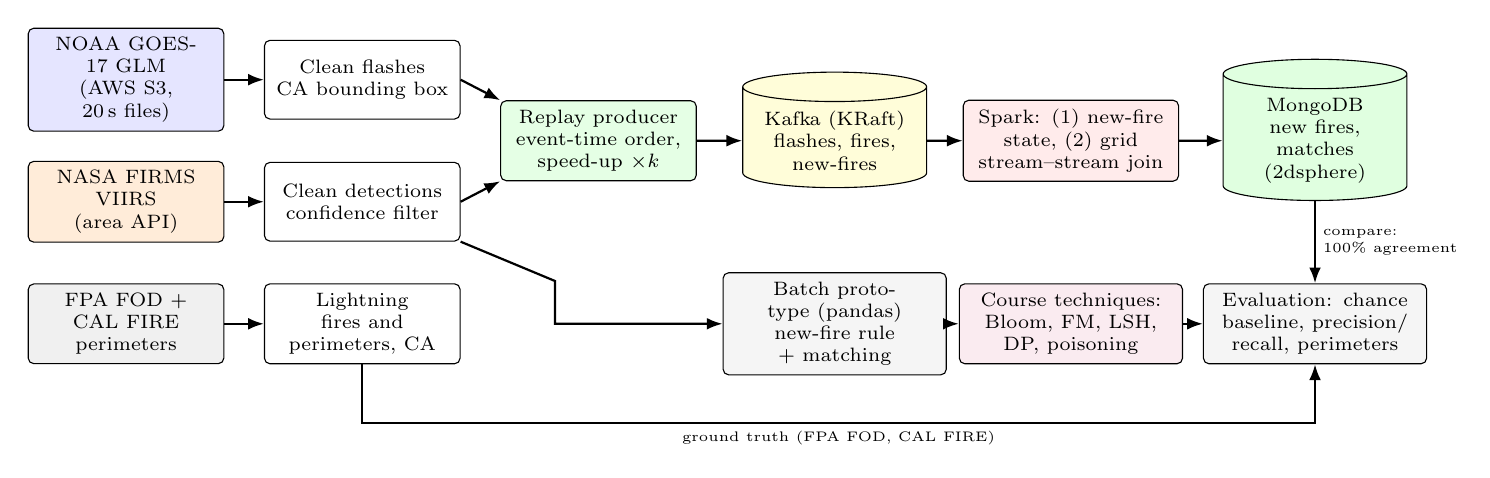
\begin{tikzpicture}[
  box/.style={draw, rounded corners=2pt, align=center, font=\scriptsize, minimum height=1.0cm, text width=2.25cm, fill=#1},
  box/.default=white,
  db/.style={draw, cylinder, shape border rotate=90, aspect=0.16, align=center, font=\scriptsize, minimum height=1.15cm, text width=2.1cm, fill=#1},
  db/.default=white,
  arr/.style={-{Latex[length=2mm]}, thick},
  lbl/.style={font=\tiny, fill=white, inner sep=1.5pt}
]
% sources and cleaning (columns 1-2)
\node[box=blue!10]   (glm)   at (0, 0)    {NOAA GOES-17 GLM\\(AWS S3, 20\,s files)};
\node[box=orange!15] (firms) at (0,-1.55)  {NASA FIRMS VIIRS\\(area API)};
\node[box=gray!12]   (fod)   at (0,-3.1)  {FPA FOD +\\CAL FIRE perimeters};
\node[box] (gcsv) at (3,0)     {Clean flashes\\CA bounding box};
\node[box] (fcsv) at (3,-1.55)  {Clean detections\\confidence filter};
\node[box] (tcsv) at (3,-3.1)  {Lightning fires and\\perimeters, CA};
% streaming path (columns 3-6)
\node[box=green!10] (prod)  at (6,-0.775)  {Replay producer\\event-time order,\\speed-up $\times k$};
\node[db=yellow!15] (kafka) at (9,-0.775)  {Kafka (KRaft)\\flashes, fires,\\new-fires};
\node[box=red!8, text width=2.5cm] (spark) at (12,-0.775) {Spark: (1) new-fire\\state, (2) grid\\stream--stream join};
\node[db=green!12]  (mongo) at (15.1,-0.775) {MongoDB\\new fires, matches\\(2dsphere)};
% batch prototype and evaluation (bottom row)
\node[box=gray!8, text width=2.6cm] (proto) at (9,-3.1)    {Batch prototype (pandas)\\new-fire rule + matching};
\node[box=gray!8, text width=2.6cm] (eval)  at (15.1,-3.1) {Evaluation: chance\\baseline, precision/\\recall, perimeters};
\node[box=purple!8, text width=2.6cm] (course) at (12,-3.1) {Course techniques:\\Bloom, FM, LSH,\\DP, poisoning};
% arrows
\draw[arr] (glm) -- (gcsv);
\draw[arr] (firms) -- (fcsv);
\draw[arr] (fod) -- (tcsv);
\draw[arr] (gcsv.east) -- (prod.north west);
\draw[arr] (fcsv.east) -- (prod.south west);
\draw[arr] (prod) -- (kafka);
\draw[arr] (kafka) -- (spark);
\draw[arr] (spark) -- (mongo);
\draw[arr] (fcsv.south east) -- ++(1.2,-0.5) |- (proto.west);
\draw[arr] (proto) -- (course);
\draw[arr] (course) -- (eval);
\draw[arr] (tcsv.south) -- ++(0,-0.75) -| node[lbl, pos=0.25, below=1pt]{ground truth (FPA FOD, CAL FIRE)} (eval.south);
\draw[arr] (mongo) -- node[lbl, right=1pt, align=left]{compare:\\100\% agreement} (eval);
\end{tikzpicture}
\caption{Flow schematic of the pipeline. Top: ingestion and streaming path (Kafka $\rightarrow$ Spark $\rightarrow$ MongoDB). Bottom: the batch prototype, the course techniques applied to its output, and evaluation against the chance baseline and two ground truths.}
\label{fig:flow}
\end{figure*}

\subsection{New-Fire Rule}
A satellite fire detection usually belongs to a fire that is already burning. We call a detection a \emph{new fire} if no other detection occurred within $r = 5$\,km in the preceding 7 days. Detections are processed in time order, and simultaneous pixels from the same overpass count only once, so a fire that first appears as several adjacent pixels yields one new fire. Data from Aug 8--14 serve only as history, and new fires are counted from Aug 15. The radius is set to 5\,km rather than 2\,km so that the spreading edge of a large fire is not mistaken for a new ignition (Section~\ref{sec:tuning}).

\subsection{Spatio-Temporal Matching}
A new fire at location $x_f$ and time $t_f$ is attributed to lightning if at least one flash $(x_g, t_g)$ satisfies
\begin{equation}
d(x_f, x_g) \le D \quad\text{and}\quad 0 \le t_f - t_g \le T,
\end{equation}
where $d$ is the distance on an equirectangular projection centred at 37$^\circ$N, which is accurate to a few percent across California. Our defaults are $D = 5$\,km and $T = 48$\,h. The prototype indexes flashes with a k-d tree and checks the time condition on the spatial candidates.

\subsection{Chance Baseline}
Lightning was dense during the siege, so some matches occur by coincidence. Our first baseline shuffled flash \emph{times} while keeping their locations. It gave a chance match rate of 72\% against a real rate of 44\%, which would imply that real lightning is \emph{worse} than random. We traced the cause to the timing: real lightning was concentrated on Aug 16--17, while most new fires appeared on Aug 18--22, and shuffling spread flashes evenly across all six days, closer to the later fires. We replaced it with a \emph{spatial-shift} baseline that keeps every flash's real time but translates the whole lightning field by 50--100\,km in a random direction (three shifts per setting). This keeps the temporal structure and the spatial clustering of the storms but breaks the link between a fire and the flash at its location.

\subsection{Validation Against Ground Truth}
A pipeline fire matches a recorded FPA FOD fire if it lies within 5\,km of the recorded point of origin and within two days of the recorded discovery date. \emph{Precision} is the share of flagged fires that match a recorded lightning fire. \emph{Recall} is the share of recorded lightning fires that were flagged, reported both for all fires and for fires of at least 10 acres, since smaller fires are often below what VIIRS can detect. We report F1 as their harmonic mean.

\subsection{Streaming Implementation}
\textbf{Kafka.} The replay producer merges flashes and detections into one event-time-ordered sequence and publishes them as JSON to two topics with three partitions each. All fire messages share one key, so they stay in order in one partition. A warm-up phase first sends the 1,201 detections of Aug 8--14 to fill the new-fire state, and a sequence number carries the prototype's order for detections from the same overpass. A speed-up factor $k$ compresses event time: at $k = 3600$, one hour of 2020 data is sent per second. Each message carries its send time so that end-to-end latency can be measured. Kafka exposes two listeners, one for clients on the host and one for containers on the Docker network.

\textbf{Spark: new-fire detector.} The first query applies the new-fire rule to the raw detection stream. It copies each detection into its $3 \times 3$ block of grid cells at least 5\,km wide and keeps, for each cell, the detections of the last 7 days in Spark's checkpointed state (\texttt{applyInPandasWithState}). A detection is new if nothing in its own cell's state lies within 5\,km and earlier. New fires go to a \texttt{new-fires} Kafka topic and to MongoDB. Two queries are needed because Spark limits chaining a custom stateful operator into a stream--stream join. The per-cell logic has no Spark dependencies, so an offline test replays the detections in 1, 50, 200 and 5,000 micro-batches; every run yields the prototype's 139 new fires.

\textbf{Spark: lightning join.} The second query reads the \texttt{new-fires} and flash topics and parses the JSON. It assigns each event to a grid cell slightly larger than $D$ in each direction, then replicates each flash into its $3 \times 3$ neighbourhood of cells. The stream--stream inner join then uses an equality condition on the cell plus the event-time range condition $t_f - T \le t_g \le t_f$, followed by an exact distance filter. Any flash within $D$ of a fire must fall in one of the nine cells around the fire, so the grid loses no matches while avoiding a cross product. Event-time watermarks of $T{+}1$\,h on flashes and 1\,h on fires let Spark discard join state that can no longer match. Results are written to MongoDB every five seconds through the MongoDB Spark connector.

\textbf{MongoDB.} Flashes are stored as GeoJSON points with a 2dsphere index, optionally combined with the flash time. The per-fire query asks for flashes within $D$ km (a spherical cap) and inside the time window.

\subsection{Course Techniques}\label{sec:coursemethods}
All five techniques run on the same data and default parameters ($D = 5$\,km, $T = 48$\,h, $r = 5$\,km) and are compared against the exact methods above.

\textbf{Bloom filter for new-fire detection.} The exact new-fire rule keeps every past detection in a k-d tree, so its memory grows with the stream. Instead, we process detections once in time order, as a stream, and store keys of the form (2.5\,km grid cell, day). A detection is new if no key from the 21 grid cells that can lie within 5\,km, over the current and previous 7 days, has been seen; it then inserts its own key. This makes 200 membership tests per event. We store keys either in an exact Python set or in a Bloom filter sized for target false-positive rates of 1\%, 0.1\%, and 0.01\%, using double hashing~\cite{kirsch2006lesshashing}. Because a Bloom filter has no false negatives, an error can only turn a new fire into ``not new''.

\textbf{Flajolet--Martin.} To summarize storm footprint in bounded memory, we estimate the number of distinct 1\,km grid cells struck by lightning each day. Each cell id is hashed with 64 salted hash functions; for each we keep the longest run of trailing zeros $R$. Estimates $0.794 \cdot 2^{\bar R}$ are averaged over groups of 8 functions~\cite{durand2003loglog}, and the median of the 8 group estimates is reported~\cite{leskovec2020mmds}.

\textbf{Locality-sensitive hashing.} As an alternative to the k-d tree, we index flash locations with p-stable LSH~\cite{datar2004pstable}: each hash is $\lfloor (\mathbf{a}\cdot\mathbf{x} + b)/w \rfloor$ with Gaussian $\mathbf{a}$, uniform $b$, and bucket width $w = 2D = 10$\,km. Each of $L$ tables concatenates $k$ hashes. A fire's candidates are the flashes sharing a bucket in any table; candidates are then filtered exactly by distance and time. We vary $k \in \{1, 2\}$ and $L \in \{1, 2, 4, 8, 16\}$.

\textbf{Differential privacy.} The data are public and contain no personal information, so this is a demonstration of how derived statistics could be released if the inputs were sensitive (for example, fire reports from private landowners). We release the number of lightning-attributed new fires per day and per 1$^\circ$ grid cell with the Laplace mechanism~\cite{dwork2006calibrating}. Adding or removing one fire changes one count by one, so the sensitivity is 1 and the noise scale is $1/\varepsilon$. Rounding and clipping at zero are post-processing and preserve the guarantee. We report the mean absolute error over 1,000 releases for $\varepsilon \in \{0.1, 0.5, 1, 2, 5\}$.

\textbf{Data poisoning.} Lightning data could be corrupted by sensor artefacts or deliberate injection. We add fake flashes, uniformly distributed over the lightning data's area and time span, equal to 10\%, 25\%, 50\%, and 100\% of the real flash count (three random seeds each), and recompute attribution and its precision against FPA FOD. As a simple defence, we compare the default rule ($\geq$1 flash in the window) with a stricter rule ($\geq$3 flashes).

%% ===================================================================
\section{Results}

\subsection{Batch Prototype}
With the default parameters, 159 new fires appeared from Aug 15 onward. Of these, 139 fell within the time span the lightning data can cover, and 65 of those (47\%) had at least one candidate flash. For matched fires, the median distance to the nearest flash was 1.8\,km and the median lag from flash to detection was 20.1\,h, which agrees with the holdover times reported in the literature~\cite{moris2023holdover,kalashnikov2023liw}.

\subsection{Chance Baseline and Parameter Tuning}\label{sec:tuning}
All 12 combinations of $D \in \{5, 10\}$\,km, $T \in \{48, 96, 168\}$\,h and new-fire radius $r \in \{2, 5\}$\,km matched more new fires with real lightning than with the shifted baseline, with ratios of 1.12--1.50 (Table~\ref{tab:tuning}). The best ratio came from the tightest setting ($D = 5$\,km, $T = 48$\,h, $r = 5$\,km): 47\% real versus 31\% chance. Widening $D$ or $T$ raised both rates, but the chance rate rose faster.

\begin{table}[!t]
\caption{Real vs.\ Chance Match Rate (Selected Settings)}
\label{tab:tuning}
\centering
\small
\begin{tabular}{@{}rrrrrrr@{}}
\toprule
$D$ & $T$ & $r$ & New & Real & Chance & Ratio \\
(km) & (h) & (km) & fires & & & \\
\midrule
\textbf{5} & \textbf{48} & \textbf{5} & \textbf{139} & \textbf{47\%} & \textbf{31\%} & \textbf{1.50} \\
5 & 48 & 2 & 305 & 38\% & 26\% & 1.47 \\
5 & 96 & 5 & 151 & 54\% & 39\% & 1.37 \\
10 & 48 & 2 & 305 & 44\% & 34\% & 1.29 \\
10 & 48 & 5 & 139 & 51\% & 42\% & 1.20 \\
10 & 168 & 5 & 159 & 62\% & 55\% & 1.12 \\
\bottomrule
\end{tabular}
\end{table}

\subsection{Precision and Recall Against FPA FOD}
Fig.~\ref{fig:pr} shows precision against recall for fires of at least 10 acres over $D \in \{2, 5, 10\}$\,km and $T \in \{24, 48, 96, 168\}$\,h. Without the lightning filter, only 23\% of new fires matched a recorded lightning fire. Every setting with the filter did better, at 33--40\%. Three patterns stand out:
\begin{itemize}
\item \textbf{$D = 2$\,km is too tight.} Overall recall fell to 4--7\%, consistent with GLM's roughly 8\,km pixel size.
\item \textbf{$T = 48$\,h is the best trade-off.} Moving from 24 to 48\,h almost doubled recall at the same precision. Longer windows added little recall and lowered precision, so most lightning fires were detected within two days.
\item \textbf{$D = 5$ and 10\,km perform alike.} F1 was 0.23 and 0.24 at $T = 48$\,h; the best F1 was 0.25 at $D = 10$\,km, $T = 96$\,h. These differences amount to a few fires out of 242. We keep $D = 5$\,km because it also gave the strongest signal over chance.
\end{itemize}

\begin{figure}[!t]
\centering
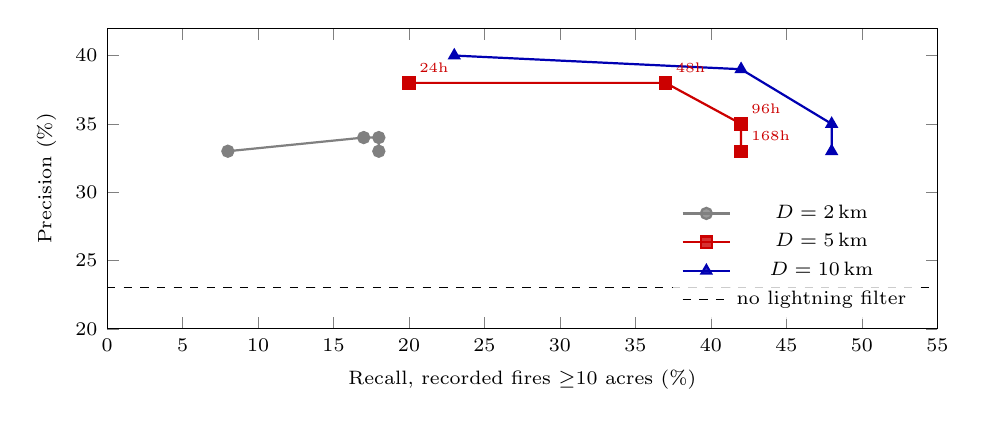
\begin{tikzpicture}
\begin{axis}[
  width=\columnwidth, height=5.4cm,
  xlabel={Recall, recorded fires $\geq$10 acres (\%)},
  ylabel={Precision (\%)},
  xmin=0, xmax=55, ymin=20, ymax=42,
  legend style={at={(0.98,0.03)},anchor=south east,font=\scriptsize,draw=none,fill=white,fill opacity=0.8,text opacity=1},
  tick label style={font=\scriptsize}, label style={font=\scriptsize},
  every node near coord/.append style={font=\tiny},
]
\addplot[gray, mark=*, thick] coordinates {(8,33) (17,34) (18,34) (18,33)};
\addplot[red!80!black, mark=square*, thick, nodes near coords, point meta=explicit symbolic, every node near coord/.append style={anchor=south west}] coordinates {(20,38)[24h] (37,38)[48h] (42,35)[96h] (42,33)[168h]};
\addplot[blue!70!black, mark=triangle*, thick] coordinates {(23,40) (42,39) (48,35) (48,33)};
\addplot[black, dashed, domain=0:55] {23};
\legend{$D=2$\,km, $D=5$\,km, $D=10$\,km, no lightning filter}
\end{axis}
\end{tikzpicture}
\caption{Precision vs.\ recall against FPA FOD for each distance threshold $D$. Points along each line are $T = 24, 48, 96, 168$\,h (labelled for $D = 5$\,km).}
\label{fig:pr}
\end{figure}

At the default setting, the filtered pipeline flagged 65 fires, with precision 38\%, recall 16\% for all recorded fires and 37\% for fires of at least 10 acres (F1 = 0.23), compared with 23\%, 19\%, 48\%, and 0.21 for all 139 new fires without the filter. The filter therefore trades some recall for a 1.7$\times$ gain in precision. Overall recall is low mainly because 75\% of recorded lightning fires were smaller than 10 acres.

\subsection{Largest Recorded Fires}
Table~\ref{tab:named} checks the 15 largest FPA FOD lightning fires discovered Aug 15--22. Twelve were detected as new fires and eight were attributed to lightning. Those eight cover 1.14 of the 2.05 million acres (56\%), including Doe, the largest fire in the window and the origin of the August Complex. Four large fires (Hopkins, Claremont, Dome, Glade) were detected but had no flash within 5\,km and 48\,h. Castle, Tatham, and Rattlesnake were not detected as new fires near their recorded points of origin.

\begin{table}[!t]
\caption{The 15 Largest Recorded Lightning Fires, Aug 15--22, 2020}
\label{tab:named}
\centering
\footnotesize
\setlength{\tabcolsep}{3pt}
\begin{tabular}{@{}llrcc@{}}
\toprule
Fire & Complex & Acres & New fire & Lightning \\
\midrule
Doe & August & 589,368 & yes & yes \\
Hopkins & August & 328,363 & yes & no \\
Claremont & North & 318,776 & yes & no \\
Hennessey & LNU Lightning & 305,651 & yes & yes \\
Castle & SQF & 174,178 & no & no \\
W-5 Cold Springs & -- & 84,817 & yes & yes \\
Wallbridge & LNU Lightning & 55,209 & yes & yes \\
SHF Elkhorn & August & 51,577 & yes & yes \\
Dome & -- & 43,273 & yes & no \\
Sheep & North & 29,570 & yes & yes \\
Glade & August & 26,197 & yes & no \\
Tatham & August & 14,457 & no & no \\
Hull & August & 12,284 & yes & yes \\
Bear & North & 12,154 & yes & yes \\
Rattlesnake & -- & 8,419 & no & no \\
\midrule
\multicolumn{2}{@{}l}{Total} & 2,054,293 & 12/15 & 8/15 \\
\bottomrule
\end{tabular}
\end{table}

\subsection{Broader Evaluation and a Second Ground Truth}\label{sec:broad}
With lightning data for Aug 21--25, the same rules were re-run over Aug 15--25 (Table~\ref{tab:broad}). The original window reproduces Section~5.3 exactly. Over the longer window the lightning filter keeps precision at 38--40\% against 22--23\% without it, and recall for fires of at least 10 acres stays at 37\%. Only 5 of the 20 new fires on Aug 23--25 matched lightning; large siege fires were still spreading, so more of the ``new'' detections may be new parts of existing fires.

\begin{table}[!t]
\caption{FPA FOD Validation over Three Windows}
\label{tab:broad}
\centering
\footnotesize
\setlength{\tabcolsep}{3pt}
\begin{tabular}{@{}lrrr@{}}
\toprule
 & Aug 15--22 & Aug 15--25 & Aug 23--25 \\
\midrule
FPA FOD fires ($\geq$10 acres) & 242 (60) & 268 (65) & 26 (5) \\
New fires flagged & 139 & 159 & 20 \\
Lightning-matched & 65 & 70 & 5 \\
Precision, all / matched & 23 / 38\% & 22 / 39\% & 15 / 40\% \\
Recall $\geq$10 ac., all / matched & 48 / 37\% & 48 / 37\% & 40 / 40\% \\
F1, all / matched & 0.21 / 0.23 & 0.20 / 0.22 & 0.13 / 0.13 \\
\bottomrule
\end{tabular}
\end{table}

Against CAL FIRE perimeters, a detection counts if it lies inside a perimeter or within 1\,km of its edge, and recall is measured on the 18 lightning fires of at least 1,000 acres (Table~\ref{tab:perim}). The lightning filter lifts precision from 46\% to 76\%, the same 1.7$\times$ gain as against FPA FOD; precision is higher because a detection anywhere on a fire counts, not just near its recorded origin. Sixteen of the 18 large lightning fires were detected as new fires; only Rattlesnake (8,309 acres) and Moraine (1,301 acres) were not. All four of the siege's best-known complexes were detected and matched to lightning within one to two days of the Aug 16--17 storms: August (13 of 16 new fires inside it matched), LNU (Hennessey, Walbridge and Meyers), SCU (7 of 9), and CZU (3 of 4). FPA FOD has no records for the SCU and CZU complexes, so perimeters are the only ground truth for two of the siege's largest fires.

\begin{table}[!t]
\caption{CAL FIRE Perimeters as Ground Truth, Aug 15--25}
\label{tab:perim}
\centering
\footnotesize
\setlength{\tabcolsep}{3pt}
\begin{tabular}{@{}lrr@{}}
\toprule
 & All new fires & Lightning-matched \\
\midrule
Fires flagged & 159 & 70 \\
Inside any 2020 perimeter & 53\% & 77\% \\
Inside a lightning fire (precision) & 46\% & 76\% \\
Large lightning fires detected & 16 of 18 & 14 of 18 \\
\quad by acres burned & 100\% & 96\% \\
\bottomrule
\end{tabular}
\end{table}

\subsection{Streaming Correctness and Performance}
We replayed all 92,594 events for Aug 15--22 (60,803 flashes and 31,791 nominal/high-confidence detections) at three speeds, after the 1,201 warm-up detections. At every speed, the detector found exactly the prototype's 139 new fires and the join found the same 65 matched fires (100\% agreement), so the grid state, bucketing and watermarks lose nothing. Table~\ref{tab:bench} and Fig.~\ref{fig:bench} summarize performance on a single laptop. Detecting a new fire took a median of 3.7--5.3\,s, about one 5\,s micro-batch. Median end-to-end latency, from the later of the fire and flash messages entering Kafka to the match being written, was 7.1--7.5\,s because each fire passes through two micro-batch steps; with the new-fire rule applied after the stream, the join alone had a median of 3.3--6.7\,s. The matcher now processes only flashes and new fires (60,942 events) and peaked at 30,959 events/s; the detector processed all 32,992 detections at up to 7,653 per second. The Python producer remained the bottleneck; its maximum of 34,453 events/s, against 15,215 in an earlier run, most likely reflects a different Python setup. For comparison, the real event rate in this period averaged about 0.13 events/s.

\begin{table}[!t]
\caption{Streaming Benchmarks (92,594 Events, New-Fire Detection in the Stream)}
\label{tab:bench}
\centering
\footnotesize
\setlength{\tabcolsep}{2.5pt}
\begin{tabular}{@{}lrrrrc@{}}
\toprule
Replay & Producer & Matcher & Detect. & End-to-end (s) & Agree- \\
speed & (ev/s) & peak (ev/s) & (s) & median / p95 & ment \\
\midrule
3,600$\times$ & 490 & 16,405 & 3.7 & 7.5 / 9.4 & 100\% \\
36,000$\times$ & 4,880 & 25,669 & 3.8 & 7.5 / 9.2 & 100\% \\
max & 34,453 & 30,959 & 5.3 & 7.1 / 7.6 & 100\% \\
\bottomrule
\end{tabular}
\end{table}

\begin{figure}[!t]
\centering
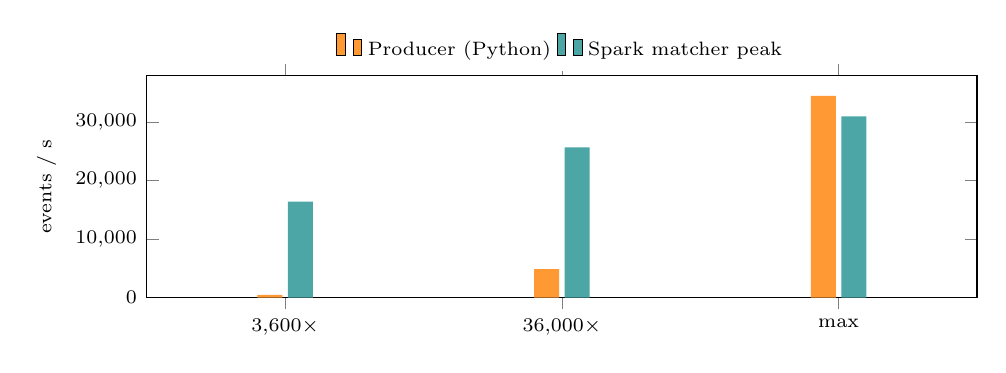
\begin{tikzpicture}
\begin{axis}[
  width=\columnwidth, height=4.4cm,
  ybar, bar width=9pt,
  symbolic x coords={3600x,36000x,max},
  xtick=data, xticklabels={3{,}600$\times$,36{,}000$\times$,max},
  ylabel={events / s}, ymin=0, enlarge x limits=0.25,
  legend style={at={(0.5,1.02)},anchor=south,legend columns=2,font=\scriptsize,draw=none},
  tick label style={font=\scriptsize}, label style={font=\scriptsize},
  scaled y ticks=false,
]
\addplot[fill=orange!80,draw=none] coordinates {(3600x,490) (36000x,4880) (max,34453)};
\addplot[fill=teal!70,draw=none] coordinates {(3600x,16405) (36000x,25669) (max,30959)};
\legend{Producer (Python), Spark matcher peak}
\end{axis}
\end{tikzpicture}
\caption{Throughput by replay speed. The matcher sees only flashes and new fires (60,942 events), so its peak is not directly comparable with the producer's rate over all events.}
\label{fig:bench}
\end{figure}

\subsection{MongoDB and Snowflake Geospatial Queries}
For each of the 139 new fires, we queried MongoDB for flashes within 5\,km and the preceding 48\,h (Table~\ref{tab:mongo}). Without an index, every query scanned all 60,803 flashes (median 36.6\,ms). A 2dsphere index reduced this to 10 documents examined and 0.57\,ms, about 64$\times$ faster; a compound index with time examined 6 documents at a similar speed. All three configurations returned the same 65 matched fires as the prototype and the stream, and building either index took 0.17\,s. We ran the same query in the Snowflake data warehouse (X-Small warehouse, result cache disabled) with \texttt{ST\_DWITHIN} on geography points~\cite{snowflakegeo}. It found the same 65 matched fires. One join over all new fires took a median of 521\,ms (120\,ms of execution), and a lookup for one fire took 346\,ms, about 600 times slower than the indexed MongoDB lookup. The warehouse suits batch analysis over many fires, and MongoDB suits per-event lookups inside the stream. An X-Small warehouse bills one credit per hour, by the second with a 60\,s minimum each time it resumes, so occasional queries cost little but a warehouse kept running for per-event lookups would not.

\begin{table}[!t]
\caption{Per-Fire Query Time (MongoDB: 139 Queries; Snowflake: 3 Runs)}
\label{tab:mongo}
\centering
\footnotesize
\setlength{\tabcolsep}{3pt}
\begin{tabular}{@{}lrrr@{}}
\toprule
System / index & Median (ms) & p95 (ms) & Docs examined \\
\midrule
MongoDB, no index & 36.64 & 41.03 & 60,803 \\
MongoDB, 2dsphere & 0.57 & 0.72 & 10 \\
MongoDB, 2dsphere + time & 0.56 & 0.70 & 6 \\
Snowflake, X-Small & 346 & -- & -- \\
\bottomrule
\end{tabular}
\end{table}

%% ===================================================================
\section{Course Techniques: Results}\label{sec:course}

\subsection{Bloom Filter}
The grid-and-day version of the new-fire rule found 139 new fires from Aug 15 onward, all of which the exact k-d tree rule also found (159 fires); the coarser cells and day buckets make it slightly more conservative. Table~\ref{tab:bloom} compares the exact set with Bloom filters. At a 0.01\% target rate, the Bloom filter reproduced all 139 new fires using 10.2\,KB instead of 362.3\,KB, a 36$\times$ reduction, and its memory stays fixed however long the stream runs. At a 1\% target, it missed 14 new fires. Because each event makes 200 lookups, the chance of at least one false positive per event is roughly 200 times the per-lookup rate, so the filter must be sized for the number of lookups, not only the number of items. In our pure-Python implementation, hashing made the Bloom filter slower per event (27--34\,$\mu$s vs.\ 5\,$\mu$s); the benefit is memory, not speed.

\begin{table}[!t]
\caption{Streaming New-Fire Detection: Exact Set vs.\ Bloom Filter}
\label{tab:bloom}
\centering
\small
\setlength{\tabcolsep}{3.5pt}
\begin{tabular}{@{}lrrrrr@{}}
\toprule
Store & Target & $k$ & Memory & New & Missed \\
 & FP rate & & (KB) & fires & \\
\midrule
Exact set & -- & -- & 362.3 & 139 & -- \\
Bloom & 1\% & 7 & 5.1 & 125 & 14 \\
Bloom & 0.1\% & 10 & 7.7 & 138 & 1 \\
Bloom & 0.01\% & 13 & 10.2 & 139 & 0 \\
\bottomrule
\end{tabular}
\end{table}

\subsection{Flajolet--Martin}
Table~\ref{tab:fm} compares the sketch with exact counts of distinct 1\,km cells struck each day. The mean absolute relative error was 8.8\%, with a range of $-20.0\%$ to $+10.1\%$, using 64 small counters instead of a set of up to 11,482 cell ids. The sketch correctly shows that the storm footprint more than tripled from Aug 15 to Aug 16--17 and collapsed by Aug 20.

\begin{table}[!t]
\caption{Distinct Lightning-Struck 1\,km Cells per Day}
\label{tab:fm}
\centering
\small
\begin{tabular}{@{}lrrrr@{}}
\toprule
Day & Flashes & Exact & FM estimate & Error \\
\midrule
Aug 15 & 5,341 & 3,576 & 3,560 & $-0.4\%$ \\
Aug 16 & 15,894 & 11,482 & 12,563 & $+9.4\%$ \\
Aug 17 & 16,489 & 11,414 & 12,563 & $+10.1\%$ \\
Aug 18 & 8,127 & 5,508 & 4,409 & $-20.0\%$ \\
Aug 19 & 13,400 & 8,114 & 8,467 & $+4.4\%$ \\
Aug 20 & 1,552 & 894 & 967 & $+8.2\%$ \\
\bottomrule
\end{tabular}
\end{table}

\subsection{Locality-Sensitive Hashing}
The exact k-d tree search found 647 fire--flash pairs for 65 matched new fires. Table~\ref{tab:lsh} shows the LSH trade-off. With one hash per table ($k = 1$), four tables already found every matched fire, but each query examined about 2,400 candidates (4\% of all flashes). With $k = 2$, buckets are narrower: four tables found all 65 matched fires and 96.4\% of pairs while examining only 107 candidates per fire (0.18\% of flashes), and 16 tables recovered every pair. Adding tables raises recall, while concatenating hashes cuts candidates; the number of candidates varies between runs because the projections are random.

\begin{table}[!t]
\caption{LSH vs.\ Exact Search (Bucket Width $w = 10$\,km)}
\label{tab:lsh}
\centering
\small
\setlength{\tabcolsep}{3.5pt}
\begin{tabular}{@{}rrrrrr@{}}
\toprule
$k$ & $L$ & Candidates & \% of & Pair & Fire \\
 & & per fire & flashes & recall & recall \\
\midrule
1 & 1 & 613 & 1.01 & 69.7\% & 98.5\% \\
1 & 4 & 2,427 & 3.99 & 99.7\% & 100\% \\
2 & 1 & 59 & 0.10 & 57.7\% & 90.8\% \\
2 & 2 & 19 & 0.03 & 87.3\% & 96.9\% \\
\textbf{2} & \textbf{4} & \textbf{107} & \textbf{0.18} & \textbf{96.4\%} & \textbf{100\%} \\
2 & 8 & 399 & 0.66 & 99.4\% & 100\% \\
2 & 16 & 323 & 0.53 & 100\% & 100\% \\
\bottomrule
\end{tabular}
\end{table}

\subsection{Differential Privacy}
The 65 attributed fires give 7 daily counts (mean 9.3) and 22 non-empty 1$^\circ$ cell counts (mean 3.0). Fig.~\ref{fig:dp} shows the relative error of the noisy release. At $\varepsilon = 1$, daily counts were off by 0.9 fires on average (9.9\% relative error), but cell counts were off by 29\%. The same absolute noise is far more damaging for fine-grained statistics with small counts: at $\varepsilon = 0.1$ the cell counts were essentially noise (209\% error). Releasing coarser aggregates, or spending more of the privacy budget, is needed for useful accuracy.

\begin{figure}[!t]
\centering
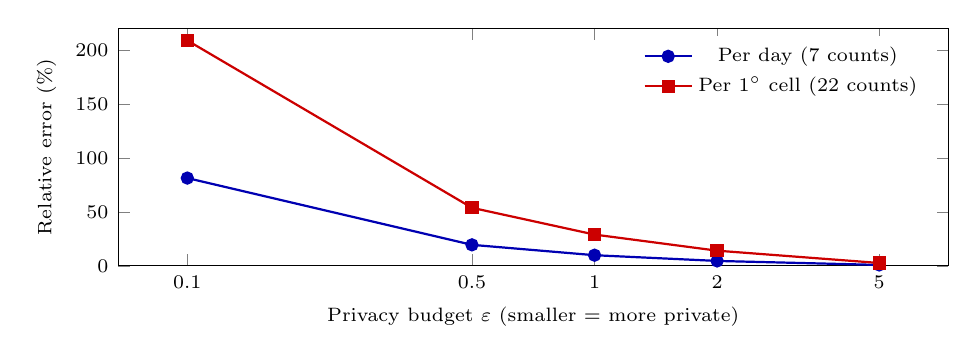
\begin{tikzpicture}
\begin{axis}[
  width=\columnwidth, height=4.6cm,
  xmode=log, log basis x=10,
  xtick={0.1,0.5,1,2,5}, xticklabels={0.1,0.5,1,2,5},
  xlabel={Privacy budget $\varepsilon$ (smaller = more private)},
  ylabel={Relative error (\%)}, ymin=0, ymax=220,
  legend style={at={(0.98,0.97)},anchor=north east,font=\scriptsize,draw=none},
  tick label style={font=\scriptsize}, label style={font=\scriptsize},
]
\addplot[blue!70!black, mark=*, thick] coordinates {(0.1,81.3) (0.5,19.5) (1,9.9) (2,4.6) (5,0.9)};
\addplot[red!80!black, mark=square*, thick] coordinates {(0.1,208.7) (0.5,53.8) (1,29.0) (2,14.1) (5,2.7)};
\legend{Per day (7 counts), Per 1$^\circ$ cell (22 counts)}
\end{axis}
\end{tikzpicture}
\caption{Accuracy cost of the Laplace mechanism on released counts of lightning-attributed fires (1,000 releases per point).}
\label{fig:dp}
\end{figure}

\subsection{Data Poisoning}
Table~\ref{tab:poison} shows that attribution is vulnerable to injected flashes. With the default $\geq$1-flash rule, fake flashes equal to the real count raised the number of flagged fires from 65 to 117 and lowered precision from 38.5\% to 27.0\%. Requiring at least three flashes made the pipeline much more robust: without poisoning it kept the same precision (38.8\%) while flagging 49 fires, and at 100\% poisoning precision fell only to 34.4\%. At 10--25\% poisoning, the stricter rule kept precision unchanged at 39.0\%. Uniform noise is a simple attack; a targeted attacker who places flashes near real fires would be harder to detect.

\begin{table}[!t]
\caption{Attribution Under Injected Fake Flashes (Mean of 3 Seeds)}
\label{tab:poison}
\centering
\small
\setlength{\tabcolsep}{4pt}
\begin{tabular}{@{}rrrrr@{}}
\toprule
Fake flashes & \multicolumn{2}{c}{$\geq$1 flash} & \multicolumn{2}{c}{$\geq$3 flashes} \\
\cmidrule(lr){2-3}\cmidrule(l){4-5}
(\% of real) & Flagged & Precision & Flagged & Precision \\
\midrule
0 & 65.0 & 38.5\% & 49.0 & 38.8\% \\
10 & 75.7 & 34.8\% & 51.3 & 39.0\% \\
25 & 85.0 & 32.6\% & 51.3 & 39.0\% \\
50 & 99.0 & 29.7\% & 55.0 & 36.4\% \\
100 & 117.3 & 27.0\% & 71.7 & 34.4\% \\
\bottomrule
\end{tabular}
\end{table}

%% ===================================================================
\section{Discussion and Limitations}
\textbf{Attribution is a signal, not proof.} A ratio of 1.5 over chance and a precision of 38\% mean that lightning proximity is informative but far from conclusive during a siege, when flashes are everywhere. Reported results should be read as candidate attributions.

\textbf{Sensor limits shape the parameters.} GLM's roughly 8\,km pixel makes distances below a few kilometres unreliable, and the twice-daily VIIRS overpass adds up to about 12\,h of detection delay. Both explain why $D = 2$\,km fails and why the median lag is about 20\,h.

\textbf{Ground truth is imperfect.} FPA FOD records a single point of origin per fire, and some complexes are recorded as one large fire. Some correct detections may therefore lie more than 5\,km from the recorded point, which would understate precision and recall. Most recorded lightning fires were also too small for VIIRS to detect. Fire perimeters show a fire's final extent, so a detection inside one may be a new spot fire on an already-burning complex rather than a separate ignition, and CAL FIRE's compilation mostly omits fires under 10 acres.

\textbf{Scope.} We studied eleven days of one extreme event in one region, on a single machine. Both rules now run in the stream, but the detector keeps exact per-cell state rather than a Bloom filter, and all fire messages share one Kafka partition to keep their order, which limits parallelism. The Bloom filter version of the rule runs as a single time-ordered pass that simulates a stream. The course techniques were evaluated in Python on one machine, so their timings are indicative only. Differential privacy is demonstrated on public, non-personal data. Latency figures assume that the host and container clocks are synchronized.

%% ===================================================================
\section{Lessons Learned, Technical Difficulties, and Best Practices}\label{sec:lessons}
\begin{itemize}
\item \textbf{Validate the baseline, not just the model.} Our first chance baseline made real lightning look worse than random. The cause was a hidden assumption that shuffling times preserves the timing between storms and fires. Any null model must preserve the structure that is not being tested.
\item \textbf{Test edge cases with real data.} A reporting script initially counted fires with no nearby detections as matched, because an empty table was silently refilled when a column was added. Synthetic test data had no unmatched fires, so tests passed. Cross-checking against an independent script (the validation step) exposed the bug.
\item \textbf{Check a streaming job against a batch reference.} Requiring 100\% agreement with the pandas prototype at every replay speed gave strong evidence that the grid bucketing, the new-fire state and the watermarks were correct.
\item \textbf{Make ordering explicit.} Pixels from one satellite overpass share a timestamp, and the prototype's unstable sort decided which of them counts as the new fire; with a stable sort the result changes slightly (140 new fires and 66 matches instead of 139 and 65). The stream carries a sequence number so that it reproduces the prototype exactly.
\item \textbf{Keep stateful logic testable.} The detector's per-cell logic has no Spark dependencies, so an offline test could replay the stream in 1 to 5,000 micro-batches without Docker and show that the answer does not depend on how Spark splits the data.
\item \textbf{Check that a data source is complete.} The NIFC perimeter layer returned only 12 small 2020 California fires and none of the siege complexes; CAL FIRE's compilation had all of them. A quick count against known events caught this.
\item \textbf{Size a Bloom filter for its lookups, not just its items.} With 200 lookups per event, a 1\% per-lookup false-positive rate silently dropped 14 of 139 new fires. A 0.01\% rate fixed this for only 5\,KB more memory.
\item \textbf{Approximate algorithms need an exact reference.} Every sketch and hash index was compared with an exact method on the same data, which turned vague claims (``LSH is faster'') into measured trade-offs (100\% fire recall at 0.18\% of comparisons).
\item \textbf{Simple rules can add robustness.} Requiring three flashes instead of one barely changed clean results but limited the precision loss under heavy poisoning to 4.4 points instead of 11.5.
\item \textbf{Mind the timing in streaming experiments.} An early run processed zero events because the Spark job stopped before the producer started. Automating the sequence (reset topics, start Spark, wait until it is listening, then replay) made the benchmarks reproducible.
\item \textbf{Container networking needs two Kafka listeners}, one advertised to the host and one to other containers. Using only \texttt{localhost} breaks clients inside Docker.
\item \textbf{Resource limits are real constraints.} Docker failed with a read-only error when the disk filled up, and lightning data must be downloaded selectively (180 files per hour). We processed files in a streaming fashion and deleted them after extraction.
\item \textbf{Environment issues cost time.} Several Python installations, missing HTTPS certificates, and cloud-synced folders that blocked version control all caused failures unrelated to the method. Pinning one interpreter and documenting setup in the repository README avoided repeats.
\end{itemize}

%% ===================================================================
\section{Conclusion and Future Work}\label{sec:future}
We built a working streaming pipeline that attributes new wildfire detections to satellite-observed lightning, validated it against a chance baseline and two ground truths, and showed that it reproduces a batch reference exactly, with both rules running in the stream and a median latency of about 7\,s. Bounded-memory and approximate techniques from the course worked well on the same data: a Bloom filter matched exact new-fire detection with 36$\times$ less memory, and LSH found every matched fire while examining a fraction of a percent of flashes. The work that remains is:
\begin{itemize}
\item \textbf{Bounded-memory state.} Replace the detector's exact per-cell state in Spark with the time-bucketed Bloom filter of Section~\ref{sec:course}, so memory stays fixed as the stream grows.
\item \textbf{Parallel fire stream.} Spread fire messages over several Kafka partitions without losing the order the new-fire rule depends on.
\item \textbf{Robustness to targeted attacks.} Test poisoning that places fake flashes near real fires, and defences based on flash energy or consistency between GOES-East and GOES-West.
\item \textbf{Broader evaluation.} Extend to the full 2020 season and test a proximity index~\cite{larjavaara2005finland} in place of a fixed $D$ and $T$.
\end{itemize}

%% ===================================================================
\section*{Use of Generative AI and Tools}
We used Claude (Anthropic) as a coding and writing assistant for the pipeline scripts, troubleshooting, and drafting this report. Team members ran every script on the real data and reviewed the outputs; all numbers come from those runs. Main tools: Python, Kafka, Spark, MongoDB, Snowflake, Docker Compose, and GitHub.

%% ===================================================================
\begin{thebibliography}{99}

\bibitem{goodman2013glm}
S.~J. Goodman \textit{et al.}, ``The GOES-R Geostationary Lightning Mapper (GLM),'' \textit{Atmospheric Research}, vol. 125--126, pp. 34--49, 2013.

\bibitem{schroeder2014viirs}
W.~Schroeder, P.~Oliva, L.~Giglio, and I.~A. Csiszar, ``The new VIIRS 375\,m active fire detection data product: Algorithm description and initial assessment,'' \textit{Remote Sensing of Environment}, vol. 143, pp. 85--96, 2014.

\bibitem{short2022fpafod}
K.~C. Short, ``Spatial wildfire occurrence data for the United States, 1992--2020 [FPA\_FOD\_20221014],'' 6th ed., Fort Collins, CO, USA: Forest Service Research Data Archive, 2022, doi: 10.2737/RDS-2013-0009.6.

\bibitem{moris2023holdover}
J.~V. Moris \textit{et al.}, ``A global database on holdover time of lightning-ignited wildfires,'' \textit{Earth System Science Data}, vol. 15, pp. 1151--1163, 2023, doi: 10.5194/essd-15-1151-2023.

\bibitem{kalashnikov2023liw}
D.~A. Kalashnikov, J.~T. Abatzoglou, P.~C. Loikith, N.~J. Nauslar, Y.~Bekris, and D.~Singh, ``Lightning-ignited wildfires in the western United States: Ignition precipitation and associated environmental conditions,'' \textit{Geophysical Research Letters}, vol. 50, no. 16, e2023GL103785, 2023, doi: 10.1029/2023GL103785.

\bibitem{rudlosky2025lightningfire}
S.~D. Rudlosky \textit{et al.}, ``Characterizing the relation between lightning and wildfires in the western United States,'' \textit{Journal of Applied Meteorology and Climatology}, vol. 64, 2025, doi: 10.1175/JAMC-D-25-0032.1.

\bibitem{larjavaara2005finland}
M.~Larjavaara, J.~Pennanen, and T.~J. Tuomi, ``Lightning that ignites forest fires in Finland,'' \textit{Agricultural and Forest Meteorology}, vol. 132, no. 3--4, pp. 171--180, 2005.

\bibitem{kreps2011kafka}
J.~Kreps, N.~Narkhede, and J.~Rao, ``Kafka: A distributed messaging system for log processing,'' in \textit{Proc. NetDB Workshop}, 2011.

\bibitem{zaharia2013dstreams}
M.~Zaharia, T.~Das, H.~Li, T.~Hunter, S.~Shenker, and I.~Stoica, ``Discretized streams: Fault-tolerant streaming computation at scale,'' in \textit{Proc. 24th ACM Symp. Operating Systems Principles (SOSP)}, 2013, pp. 423--438.

\bibitem{armbrust2018structured}
M.~Armbrust \textit{et al.}, ``Structured Streaming: A declarative API for real-time applications in Apache Spark,'' in \textit{Proc. ACM SIGMOD Int. Conf. Management of Data}, 2018, pp. 601--613.

\bibitem{yu2015geospark}
J.~Yu, J.~Wu, and M.~Sarwat, ``GeoSpark: A cluster computing framework for processing large-scale spatial data,'' in \textit{Proc. 23rd ACM SIGSPATIAL Int. Conf. Advances in Geographic Information Systems}, 2015, pp. 1--4.

\bibitem{mongodb2dsphere}
MongoDB, Inc., ``2dsphere indexes,'' MongoDB Manual. [Online]. Available: \url{https://www.mongodb.com/docs/manual/core/indexes/index-types/geospatial/2dsphere/}

\bibitem{leskovec2020mmds}
J.~Leskovec, A.~Rajaraman, and J.~D. Ullman, \textit{Mining of Massive Datasets}, 3rd ed. Cambridge, U.K.: Cambridge Univ. Press, 2020.

\bibitem{bloom1970}
B.~H. Bloom, ``Space/time trade-offs in hash coding with allowable errors,'' \textit{Communications of the ACM}, vol. 13, no. 7, pp. 422--426, 1970.

\bibitem{kirsch2006lesshashing}
A.~Kirsch and M.~Mitzenmacher, ``Less hashing, same performance: Building a better Bloom filter,'' in \textit{Proc. 14th Annu. European Symp. Algorithms (ESA)}, LNCS 4168, 2006, pp. 456--467.

\bibitem{flajolet1985}
P.~Flajolet and G.~N. Martin, ``Probabilistic counting algorithms for data base applications,'' \textit{Journal of Computer and System Sciences}, vol. 31, no. 2, pp. 182--209, 1985.

\bibitem{durand2003loglog}
M.~Durand and P.~Flajolet, ``Loglog counting of large cardinalities,'' in \textit{Proc. 11th Annu. European Symp. Algorithms (ESA)}, LNCS 2832, 2003, pp. 605--617.

\bibitem{indyk1998lsh}
P.~Indyk and R.~Motwani, ``Approximate nearest neighbors: Towards removing the curse of dimensionality,'' in \textit{Proc. 30th ACM Symp. Theory of Computing (STOC)}, 1998, pp. 604--613.

\bibitem{datar2004pstable}
M.~Datar, N.~Immorlica, P.~Indyk, and V.~S. Mirrokni, ``Locality-sensitive hashing scheme based on p-stable distributions,'' in \textit{Proc. 20th Annu. Symp. Computational Geometry (SoCG)}, 2004, pp. 253--262.

\bibitem{sweeney2002kanon}
L.~Sweeney, ``k-anonymity: A model for protecting privacy,'' \textit{Int. J. Uncertainty, Fuzziness and Knowledge-Based Systems}, vol. 10, no. 5, pp. 557--570, 2002.

\bibitem{dwork2006dp}
C.~Dwork, ``Differential privacy,'' in \textit{Proc. 33rd Int. Colloq. Automata, Languages and Programming (ICALP)}, 2006, pp. 1--12.

\bibitem{calfire2020perimeters}
California Department of Forestry and Fire Protection (CAL FIRE), Fire and Resource Assessment Program, ``California Fire Perimeters (all),'' ArcGIS feature service, accessed Nov. 2026.

\bibitem{snowflakegeo}
Snowflake Inc., ``Geospatial functions,'' Snowflake Documentation. [Online]. Available: \url{https://docs.snowflake.com/en/sql-reference/functions-geospatial}

\bibitem{dwork2006calibrating}
C.~Dwork, F.~McSherry, K.~Nissim, and A.~Smith, ``Calibrating noise to sensitivity in private data analysis,'' in \textit{Proc. 3rd Theory of Cryptography Conf. (TCC)}, 2006, pp. 265--284.

\bibitem{biggio2012poisoning}
B.~Biggio, B.~Nelson, and P.~Laskov, ``Poisoning attacks against support vector machines,'' in \textit{Proc. 29th Int. Conf. Machine Learning (ICML)}, 2012, pp. 1467--1474.

\end{thebibliography}

%% ===================================================================
\clearpage
\onecolumn
\appendices

\section{How the Rubric Criteria Are Met}
Criteria are listed in the order of the course rubric.

\noindent Repository (public): \url{https://github.com/chinmayibolisetty-cmd/wildfire-lightning-pipeline.}\\
Agile board (Trello): \url{https://trello.com/b/LEu9Qd2D/wildfire-lightning-pipeline-data-226}

\medskip
\renewcommand{\arraystretch}{1.25}
\small
\begin{tabularx}{\textwidth}{@{}>{\raggedright\arraybackslash}p{3.6cm}>{\raggedright\arraybackslash}X@{}}
\toprule
Criterion & How it is met and evidence \\
\midrule
Code walkthrough & Presented live in class from the public repository. The code is grouped as data download (\texttt{get\_glm.py}, \texttt{get\_firms.py}, \texttt{get\_fpa\_fod.py}, \texttt{get\_nifc.py}), batch prototype and evaluation (\texttt{match\_prototype.py}, \texttt{tune.py}, \texttt{validate.py}, \texttt{pr\_sweep.py}, \texttt{broad\_eval.py}), streaming and benchmarks (\texttt{replay\_producer.py}, \texttt{spark\_match.py}, \texttt{new\_fire\_state.py}, \texttt{bench.sh}), databases (\texttt{mongo\_bench.py}, \texttt{snowflake\_queries.sql}), and course techniques (\texttt{course\_techniques.py}). \texttt{results.ipynb}, with a \texttt{.py} export, shows all results. \\
Presentation skills & Assessed at the in-class presentation; the talk is planned to fit the assigned time slot. \\
Discussion / Q\&A & Assessed at the in-class presentation; we leave time for questions after the talk. \\
Demo & Planned live demo: start Kafka, MongoDB, and Spark with Docker Compose, replay the siege at 36,000$\times$ (about 19\,s), and show matches arriving in MongoDB (\texttt{bench.sh}). \\
Report & This report uses the IEEE Computer Society \LaTeX\ template and contains no code or screenshots; all figures are drawn from data. \\
Version control & Public GitHub repository above with code, data, results, and README. Commits from all four team members between Nov 12 and Nov 17, 2026, including a merged pull request (\#1) for in-stream detection and the broader evaluation. Earlier work was consolidated into a single commit on Nov 12, 2026, so commits before that date are not visible. \\
Lessons learned & Section~\ref{sec:lessons} of this report and slide 18 of the presentation. \\
Prospects of competition / publication & Results on a real, extreme event with a ground-truth evaluation could suit a student poster or abstract at a venue such as the AGU Fall Meeting or ACM SIGSPATIAL. \\
Innovation & To our knowledge, this is the first open pipeline that joins GOES GLM and VIIRS as live streams, tests the result against a chance baseline, and validates it against FPA FOD and CAL FIRE perimeters. \\
Teamwork & Commits from all four team members and a merged pull request on GitHub; shared Trello board. \\
Technical difficulty & Stream--stream spatio-temporal join with a 48\,h window, a stateful new-fire detector in Spark linked to the join through Kafka, grid bucketing with watermarks, multi-container networking, processing of about 47,500 satellite files, two ground truths, statistical validation, and five course techniques measured against exact references. \\
Practiced pair programming & Practiced in person: Chinmayi and Rachel worked side by side on the matching prototype, one writing and one reviewing the code. Other work was done individually and shared through GitHub. \\
Practiced agile / scrum (1-week sprints) & Trello board (link above) with 1-week sprint lists, a backlog, and labels for done, in-progress and to-do work. Sprints 1--7 were logged retrospectively on Nov 17, 2026 from Git history and course submissions; Sprint 8 was tracked live. \\
Slides & Slide deck (\texttt{.pptx} with animations, plus a PDF export) with the flow schematic (slide 4), lessons learned (slide 18) and the CRediT statement (slide 20). \\
Used \LaTeX & This report: IEEEtran class with the \texttt{compsoc} option, as in the Overleaf IEEE template for computer science journals; \texttt{.tex} file uploaded. \\
Creative presentation techniques & Staged click-to-reveal animations on the pipeline, method, results, demo and lessons-learned slides, and fade transitions throughout. \\
Literature survey & Section~2, organized into subsections; 25 references in IEEE style. \\
Use of streaming algorithms & Bloom filter for one-pass new-fire detection with 36$\times$ less memory than an exact set and no missed fires at a 0.01\% target rate (Table~\ref{tab:bloom}); Flajolet--Martin estimate of distinct struck cells per day with 8.8\% mean error (Table~\ref{tab:fm}). Both run as a time-ordered pass that simulates a stream; the Spark detector uses exact per-cell state. \\
Use of stream processing frameworks & Apache Kafka (KRaft; flash, fire and new-fire topics) and Spark Structured Streaming (a stateful new-fire detector and a stream--stream join with watermarks) in Docker Compose; 100\% agreement with the batch reference (139 new fires, 65 matches) and benchmarks in Table~\ref{tab:bench}. \\
Use of Locality Sensitive Hashing & p-stable LSH for the fire--flash near-neighbour search, compared with an exact k-d tree: 100\% of matched fires found while examining 0.18\% of flashes ($k = 2$, $L = 4$; Table~\ref{tab:lsh}). \\
Use of privacy techniques & Differential privacy (Laplace mechanism) for releasing counts of attributed fires per day and per 1$^\circ$ cell, with the accuracy cost measured for five values of $\varepsilon$ (Fig.~\ref{fig:dp}). The data are public and non-personal, so this is presented as a demonstration. \\
Other course tools and techniques & Data poisoning: injected fake flashes reduce precision from 38.5\% to 27.0\%; a $\geq$3-flash rule limits this to 34.4\% (Table~\ref{tab:poison}). \\
Use of new tools not used in homework & GOES GLM via public cloud storage (s3fs/xarray), NASA FIRMS API, CAL FIRE perimeter service, MongoDB 2dsphere geospatial indexes, MongoDB Spark connector, Snowflake geospatial SQL, Docker Compose for multi-container orchestration (homework used single containers), and Trello. \\
Flow schematic diagram & Fig.~\ref{fig:flow} in this report (with description in Section~\ref{sec:methods}) and slide 4 of the presentation. \\
\bottomrule
\end{tabularx}

\end{document}
